% !TEX root = ../../Thesis.tex
%%%%%%%%%%%%%%%%%%%%%%%%%%%%%%%%%%%%%%%%%%%%%%%%%%%%%%%%%%%%%%%%%%%%%%%%
\chapter{Applicazioni modellistiche della decomposizione CP}
\label{chp:cp_applications}
%%%%%%%%%%%%%%%%%%%%%%%%%%%%%%%%%%%%%%%%%%%%%%%%%%%%%%%%%%%%%%%%%%%%%%%%
\todo{migliorato}
In questo capitolo esploreremo due applicazioni della decomposizione CP di un tensore a tre indici
in due ambiti modellistici,
dove avremo modo di applicare il Teorema di Kruskal~\ref{thm:kruskal3d} e l'algoritmo Alternating
Least Squares. Nel primo esperimento il rango non sarà noto a priori e dovremo prima approssimarlo,
per poi trovare una decomposizione. Nel secondo conosceremo il rango a priori.
In entrambi gli esperimenti sarà necessario risolvere l'ambiguità del riscalamento e della
permutazione dei fattori per preservare il modello reale.

\section{Spettroscopia fluorescente}

Nella \emph{spettroscopia fluorescente}, un campione chimico è eccitato e
la luce emessa viene misurata a diverse lunghezze d'onda, risultando in una matrice di
\emph{eccitazione-emissione} (EEM) di intensità fluorescenti (si veda Figura~\ref{fig:spectroscopy}). Quando i dati EEM vengono raccolti da
diversi campioni, otteniamo un tensore a tre indici. Questi dati si possono utilizzare nella chimica
analitica per stimare le concentrazioni e gli spettri dei composti chimici a
partire da più miscele.

\begin{figure}[htbp]
	\centering
	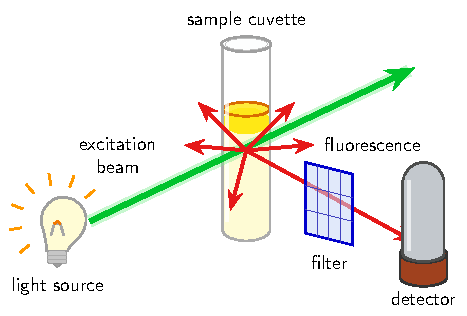
\includegraphics{Sources/Chapter4/figures/spectroscopy.pdf}
	\caption{Rappresentazione schematica di uno spettrofotometro per spettroscopia di fluorescenza.}
	\label{fig:spectroscopy}
\end{figure}

Nel dettaglio, vengono dati $ I $ campioni di soluzioni chimiche, ognuno dei quali contiene diverse sostanze
diluite in diverse concentrazioni. Il primo obiettivo è determinare il numero $ r $ delle diverse
sostanze presenti.
Il dataset che analizziamo~\cite{kolda2021eem,acar2014structure} è composto da una serie di esperimenti riportati
da~\cite{smilde2004multi}, nel quale sono presenti tre sostanze chimiche disciolte nelle soluzioni:
\begin{itemize}
	\item \emph{Valine-Tyrosine-Valine} (Val-Tyr-Val) - peptide,
	\item \emph{Tryptophan-Glycine} (Trp-Gly) - peptide,
	\item \emph{Phenylalanine} (Phe) - aminoacido.
\end{itemize}
Segnaliamo che i dati sono stati preprocessati dagli autori per riempire i dati mancanti e
sostituire le entrate negative, come spiegato in~\cite{kolda2021eem}.

Ogni campione, diciamo il numero $ i $-esimo è
successivamente eccitato da una luce in $ J $ diverse lunghezze d'onda. Per ogni lunghezza d'onda di
eccitazione, viene misurato lo spettro emesso. Diciamo che l'intensità della luce fluorescente
emessa è misurata da $ K $ diverse lunghezze d'onda. Allora per ogni $ i $ otteniamo una matrice $
	J\times K $ di eccitazione-emissione.

Quindi i dati possono essere rappresentati come un array $ I \times J \times K $, scrivibile come
\begin{equation*}
	T = \sum_{f=1}^r a_{f} \otimes b_{f} \otimes c_{f},
\end{equation*}
in componenti,
\begin{equation*}
	T_{ijk} = \sum_{f=1}^r a_{if}b_{jf}c_{kf},
\end{equation*}
dove $ a_{i,f}
$ è la concentrazione della $ f $-esima sostanza nell'$ i $-esimo campione, $ c_{k,f} $ è la frazione di protoni che la $ f $-esima
sostanza emette nella lunghezza d'onda $ k $ e $ b_{j,f} $ è l'intensità della luce incidente alla
lunghezza d'onda $ j $ moltiplicata per l'assorbimento alla lunghezza d'onda $ j $.
Il primo obiettivo è
trovare un $ r $ tale che
ogni $ f $ rappresenti una sostanza.

Il dataset analizzato contiene le misurazioni di matrici di eccitazione-emissione (EEM) per 18
campioni, ognuno dei quali consiste in una miscela dei tre composti chimici sopra (Val-Tyr-Val,
Trp-Gly e Phe). I dati sono organizzati in un tensore tridimensionale di dimensioni $ I \times  J
	\times K = 18 \times 251
	\times 21$, corrispondenti rispettivamente ai $ 18 $ campioni, alle $ 251 $ lunghezze d'onda di
emissione $(250,251, \ldots,
	500 \text{nm})$ e alle lunghezze d'onda di eccitazione $(210, 215, \ldots, 310 \text{nm})$. Una rappresentazione
tridimensionale del tensore è mostrata in Figura~\ref{fig:piled_tensor}, mentre alcune sezioni di
matrici di eccitazione-emissione sono visualizzate in Figura~\ref{fig:x_slices}.

\begin{figure}[htbp]
	\centering
	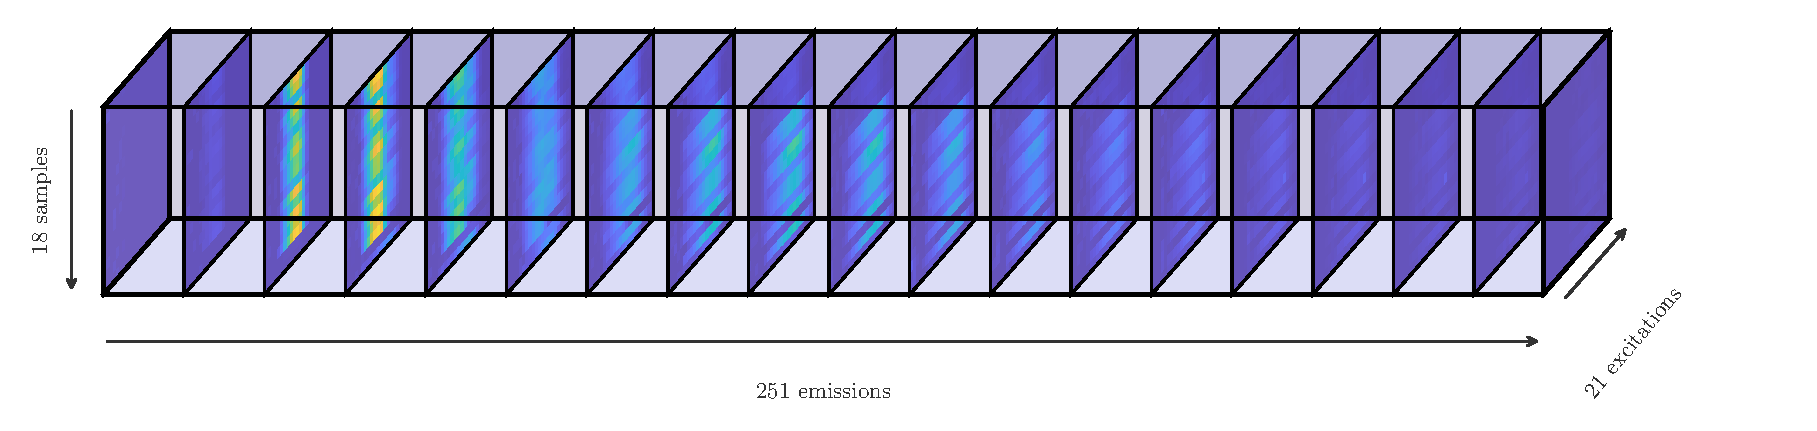
\includegraphics[width=0.85\textwidth]{Sources/Chapter4/figures/piled_tensor.pdf}
	\caption{Rappresentazione tridimensionale del tensore EEM di dimensioni $18 \times 251 \times 21$.}
	\label{fig:piled_tensor}
\end{figure}

\begin{figure}[htbp]
	\centering
	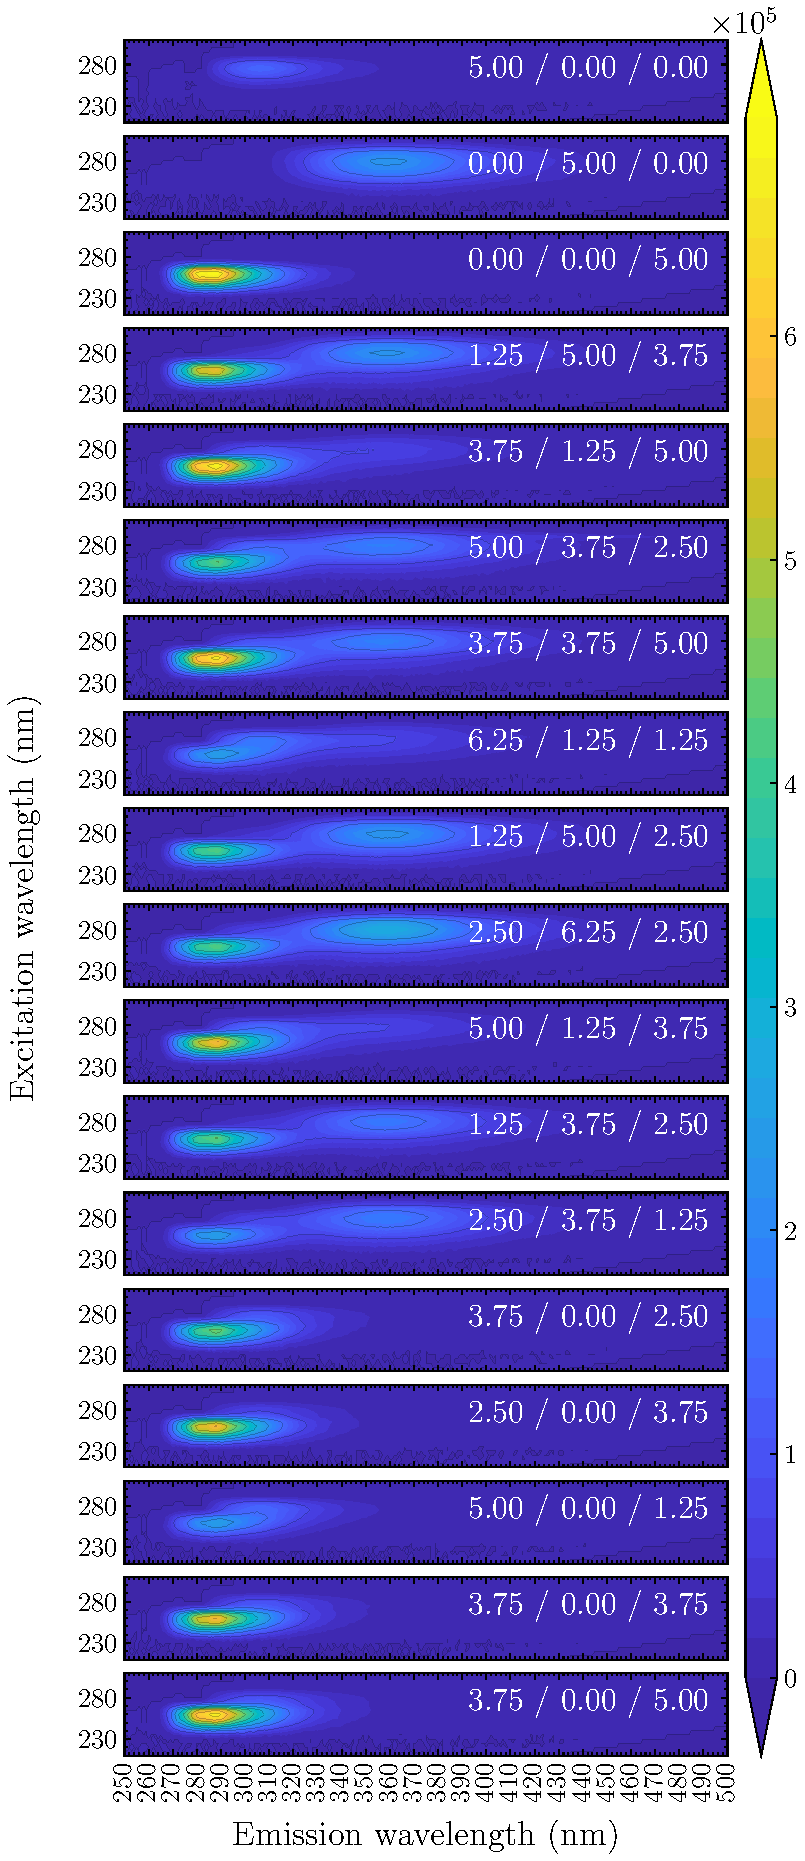
\includegraphics[width=0.60\textwidth]{Sources/Chapter4/figures/X-slices.pdf}
	\caption{Profili d'intensità di emissione-eccitazione del tensore EEM. I profili rappresentano le
		matrici EEM e corrispondono
		alle fette orizzontali del tensore, ordinate dall'alto ($ T_{1,:,:} $) al basso ($ T_{18,:,:}
		$).
		Ogni fetta è etichettata a destra con le concentrazioni dei tre composti chimici
		(Val-Tyr-Val/Trp-Gly/Phe), e copre $ 21 $ lunghezze d'onda d'eccitazione per $ 251 $ lunghezze
		d'onda di emissione.}
	\label{fig:x_slices}
\end{figure}


Cerchiamo una fattorizzazione approssimata di $ \hat{T} $ con le tecniche descritte nella \S~\ref{sec:computing_cp}. Fissata una
tolleranza $ \varepsilon $ piccola, applichiamo il procedimento
dell'Algoritmo~\ref{alg:tensor_approx}. La ricerca di $ \hat{T} $ viene ripetuta attraverso una
serie di restarts per evitare minimi locali, al termine dei quali viene restituito il tensore che
minimizza l'errore relativo $ \varepsilon_{\text{rel}} $. Nell'articolo originale~\cite{smilde2004multi} vengono anche esclusi i tensori che non sono
ragionevoli da un punto di vista fisico per rimuovere valori di $ r $ troppo piccoli. Per i nostri scopi ci limitiamo a imporre che le quantità fisiche coinvolte (concentrazioni, intensità di emissione ed eccitazione) siano non negative, per cui si scartano le decomposizioni che presentano fattori negativi.

\begin{algorithm}[htbp]
	\caption{Algoritmo di approssimazione del tensore originale.}
	\label{alg:tensor_approx}
	\begin{algorithmic}[1]
		\For{$i = 1 \dots r$}
		\Repeat
		\State $\hat{T} \gets \arg\min_{A, B, C} \nrm{T - \dsqr{A, B, C}}$ \Comment{CP ALS con restarts.}
		\Until{$\nrm{T - \hat{T}} < \varepsilon$}
		\EndFor
	\end{algorithmic}
\end{algorithm}

\begin{figure}[htbp]
	\centering
	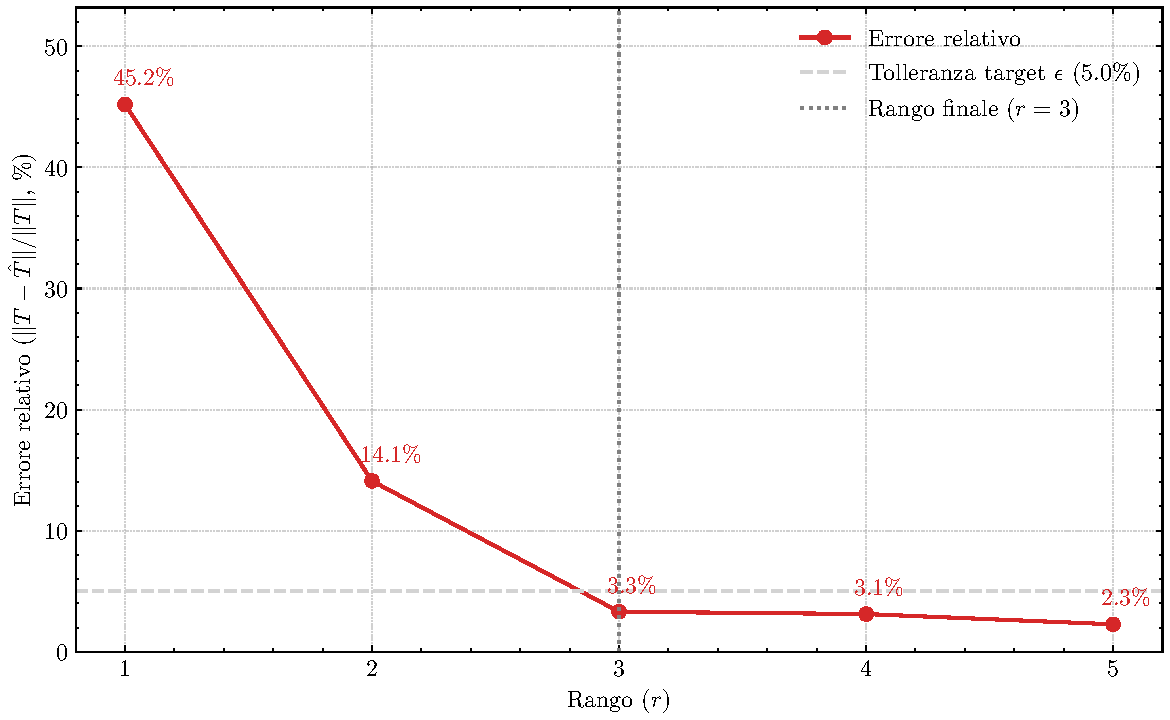
\includegraphics[width=0.7\textwidth]{Sources/Chapter4/figures/eem_cp_error_vs_rank.pdf}
	\caption{Errore relativo al variare del rango della decomposizione approssimante. Il rango
		ottimale selezionato è $r = 3$, corrispondente al superamento della tolleranza target
		$\varepsilon = 0.05$. Osserviamo che la precisione non varia di molto all'aumentare di $ r $.}
	\label{fig:eem_cp_error_vs_rank}
\end{figure}

Assumiamo ora che il rango ottimale $ r $ sia stato determinato attraverso l'euristica discussa in
\S~\ref{sec:computing_rank}. Siccome i valori di $ r $ sono relativamente piccoli,
a meno di piccole perturbazioni, l'espressione di $ \hat{T} $ come somma di elementi di rango uno
sarà unica grazie al Teorema di Kruskal~\ref{thm:kruskal3d}. Quindi, decomponendo $ \hat{T} $,
possiamo recuperare la concentrazione
di ognuna delle $ r $ sostanze in ogni soluzione, determinando i vettori $ a_{f} $ così come lo
spettro delle eccitazioni ed emissioni determinando i vettori $ b_{f} $.
La Figura~\ref{fig:eem_model} mostra i fattori calcolati e il confronto con le concentrazioni reali
delle tre sostanze, arrestando CP ALS quando la differenza dell'errore relativo tra due iterazioni
susseguenti è minore di $ 10^{-4} $. Nel grafico sono tracciati i fattori $ a_{f},b_{f},c_{f} $ della decomposizione
CP, dove ogni riga $ f  = 1,2,3 $ rappresenta una sostanza diversa (scritta in sottoimpressione). Ad
esempio, la componente $ a_1 $ sono le barre blu nella prima sottofigura in alto a sinistra, dove
notiamo che i primi due fattori di $ a_{1} $ sono nulli, che significa che la componente non è
presente nei primi due campioni. Nella colonna centrale in alto denotiamo le componenti individuali di $ b_1
$, che sono $ 256 $, con dei punti. Il terzo fattore $ c_1 $ è rappresentato nella figura in alto a
destra. Analogamente la seconda riga descrive i fattori $ a_2,b_2,c_2 $ e la terza $ a_3,b_3, c_3 $.
Nel calcolo della fattorizzazione abbiamo dovuto riscalare i fattori del tensore ottenuto da ALS per
mantenere i valori fedeli al tensore originale. Inoltre abbiamo permutato i fattori con un algoritmo
simile a quello che descriveremo nella \S~\ref{sec:num_experiment_omini}.\todo{Serve precisare
	meglio?}


\begin{figure}[htbp]
	\centering
	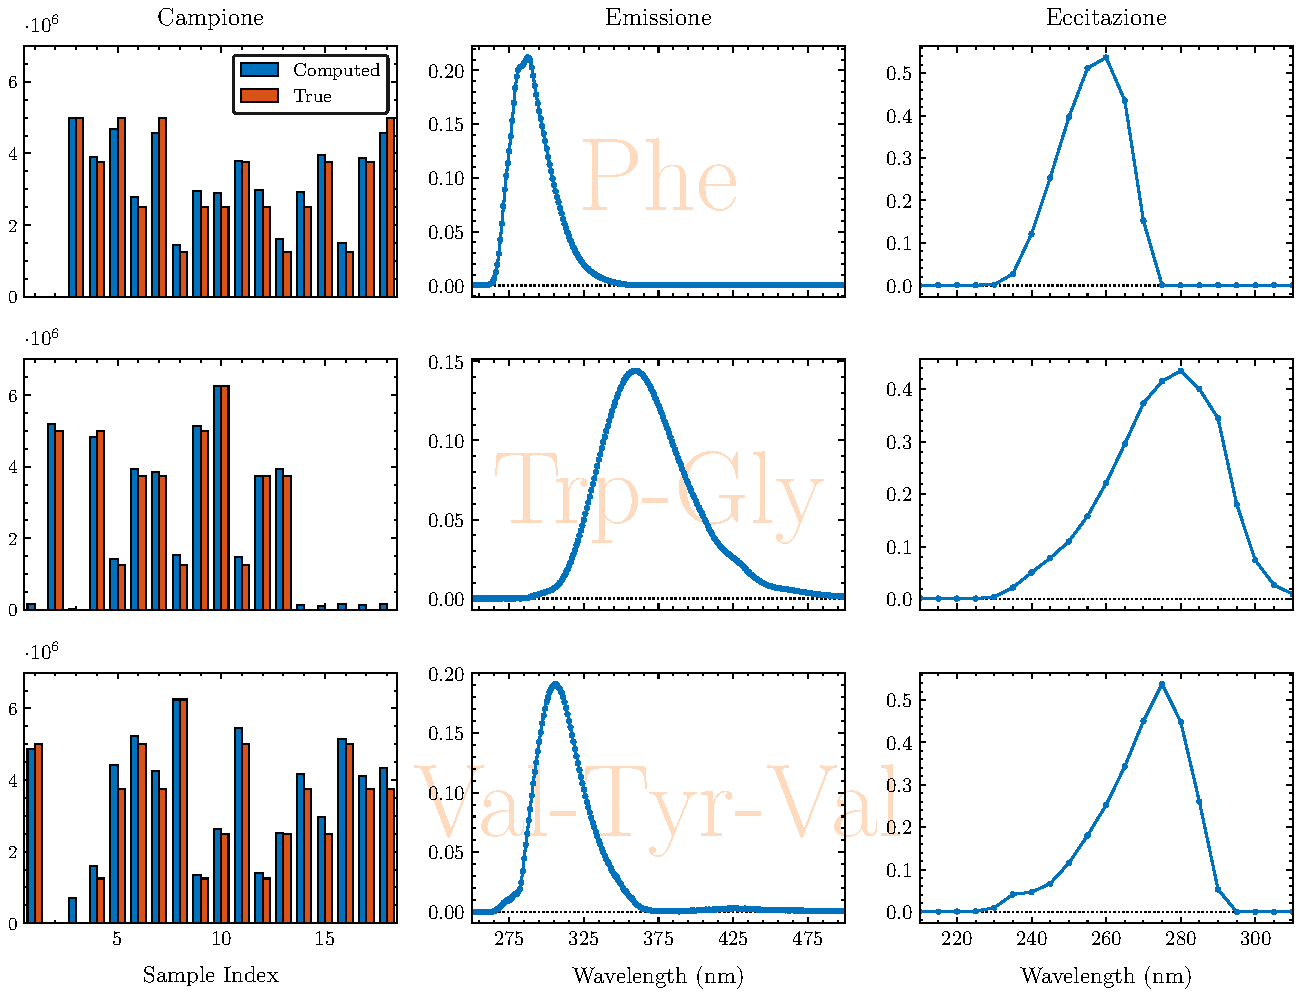
\includegraphics[width=1\textwidth]{Sources/Chapter4/figures/eem_model.pdf}
	\caption{Fattori della decomposizione CP non negativa a rango $r=3$ del tensore EEM. I diagrammi a barre a sinistra confrontano i profili di concentrazione calcolati con le concentrazioni effettive delle tre sostanze (Val-Tyr-Val, Trp-Gly, Phe).}
	\label{fig:eem_model}
\end{figure}

\pagebreak

\section{Blind source separation}

Immaginiamo una stanza affollata in cui diverse persone parlano contemporaneamente, mentre alcuni
microfoni sparsi per la sala che registrano le
conversazioni. Poiché i microfoni catturano solo la sovrapposizione delle singole voci, l'obiettivo
è elaborare le registrazioni per isolare la voce di ogni singola persona. Questo scenario è noto
nell'analisi di segnali come \emph{blind source separation}.

In questa sezione studieremo un problema simile utilizzando la decomposizione CP. In particolare, ci
concentreremo su un'applicazione nel campo delle telecomunicazioni wireless nota come \emph{blind
	deconvolution} nel modello \emph{direct-sequence code-division multiple
	access} (DS-CDMA)~\cite{sidiropoulos2000blind,de2008blind,landsberg2011tensors} che riadattiamo in
questa sezione.

Per semplicità supponiamo che $ R $ utenti mandino dei messaggi a $ I $ antenne. I messaggi arrivano
mischiati, e l'obiettivo è recuperare i segnali individuali e le posizioni degli utenti.


\begin{figure}[htbp]
	\centering
	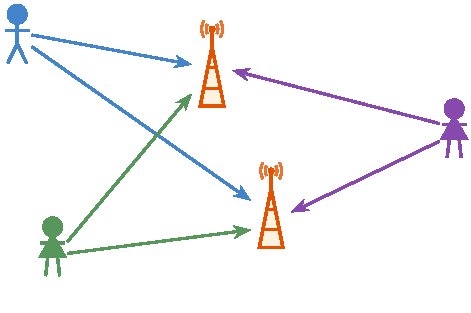
\includegraphics{Sources/Chapter4/figures/antennae.pdf}
	\caption{$R = 3$ sorgenti inviano segnali a $I = 2$ antenne.}
	\label{fig:antennae}
\end{figure}

L'utente $ r $-esimo trasmette il messaggio in un vettore di $ s_{r} = \left[ s_{1r}, \ldots, s_{Kr}
		\right]^{\top}  \in \R^{K}$, dove le entrate sono numeri reali random. Ci sono $ I $ antenne che ricevono i segnali.
Quando i segnali arrivano all'$ i $-esima antenna, il segnale ha subito distorsione
nella sua intensità e fase (anche detta \emph{fading/gain}), quindi ciò che viene ricevuto dall'antenna $
	i $-esima sono le $ IK $ quantità $ a_{ir}s_{kr} $, dove $ a_{ir} $ è il fading/gain tra l'utente $
	r $ e l'antenna $ i $.

In questo scenario si riceve un tensore (matrice) $ T \in \C^{I \times K} $ di rango $ R $ di entrate
\begin{equation*}
	T_{ik} = \sum_{r=1}^R a_{ir}s_{kr}.
\end{equation*}
L'obiettivo sarebbe recuperare i segnali $ s_{r} $, per $ 1\le r \le R $ da questa
matrice decomponendola come somma di matrici di rango uno. Sfortunatamente, questa decomposizione non è mai
unica quando $ R > 1 $. Per aggirare il problema, vengono introdotti dei ``codici'' per ``diffondere'' il segnale che
ogni utente invia per ottenere un tensore a tre indici che avrà generalmente una decomposizione
unica.\footnote{Tale spreading è comune nelle telecomunicazioni, e.g. della ridondanza è introdotta per
	compensare gli errori causati dalla corruzione dei segnali durante la trasmissione.}

Facciamo le seguenti ipotesi sulla trasmissione dei segnali: la trasmissione avviene in linea
d'aria, seguendo la strada più breve (secondo la distanza euclidea) senza incontrare ostacoli; i
simboli inviati arrivano in maniera ordinata senza sovrapposizione (esempio $ s_{k,r} $ allo stesso
tempo di $ s_{k+1,r} $). Questi comportamenti sono noti in letteratura come ICI (\emph{interchip
	interference}) e ISI (\emph{intersignal interference}).
Inoltre i segnali non subiscono rumore e non vengono memorizzati.

Per recuperare $ s_{r}
$ e $ a_{ir} $, l'$ r $-esimo utente
introduce una ridondanza in termini di codice chiamata \emph{spreading sequence} che è fissata per
ogni utente, diciamo $ c_{r} = \left[ c_{1r}, \ldots, c_{Jr} \right]^{\top} $. Vengono trasmesse simultaneamente $ J $ quantità
$ \left[ s_{kr}c_{1r}, \ldots, s_{kr}c_{Jr} \right] $, chiamate \emph{chips} al tempo $ k $, dove in
ogni entrata rappresenta la trasmissione del simbolo $ s_{kr} $ su una frequenza diversa. La
trasmissione totale sopra $ JK $ unità di tempo dell'utente $ r $-esimo sono le $ JK $ chips $
	c_{jr}s_{kr} $, $ 1 \le j \le J $, $ 1\le k \le K $ (qui $ J $ è anche detto \emph{spreading gain}).
L'antenna $ i $-esima riceve le $ JK $ quantità $ \sum_{r} a_{ir}c_{jr}s_{kr} $, per $ 1 \le j \le J
$, $ 1 \le k \le K $, dove, come sopra, $ a_{ir} $ sono i fading/gain tra l'utente $ r $ e l'antenna
$ i $. In totale, viene ricevuto un tensore $ T \in \C^{I \times J\times K} $ di rango $ R $
scrivibile in componenti come
\begin{equation}
	\label{eq:blindec_cp_components}
	T_{ijk} = \sum_{r=1}^R a_{ir}c_{jr}s_{kr},
\end{equation}
o in generale,
\begin{equation*}
	T = \sum_{r=1}^R a_{r} \otimes c_{r} \otimes s_{r}.
\end{equation*}
In altre parole, $ T = \dsqr{S,C,A} $. L'obiettivo è recuperare i segnali $ s_{r} $, per $ 1\le r\le
	R $ da questo tensore, cioè la matrice $ S $. Per farlo abbiamo bisogno che la scrittura sia
essenzialmente unica. Per il Teorema di Kruskal~\ref{thm:kruskal3d} questa decomposizione è unica se
\begin{equation*}
	\krk{A} + \krk{B} + \krk{C} \ge 2(R+1).
\end{equation*}
Per costruzione~\cite{de2008blind} le matrici $ A $ e $ C $ sono di $ k $-rango pieno con probabilità $ 1
$, mentre se i simboli trasmessi $ s_{Kr} $ appartengono ad un alfabeto finito, c'è possibilità che
$ S $ non sia di $ k $-rango pieno---c'è una possibilità che le sequenze di utenti diversi possano essere
uguali, ma questo è poco probabile per dataset più grandi. Quindi nella pratica assumiamo che $ S $
sia di $ k $-rango pieno. Questo significa che il numero di utenti che possono essere processati
simultaneamente si può considerare limitato come
\begin{equation}
	\label{eq:krk_eq_full_rank}
	\min \{I,R\} + \min \{J,R\} + \min \{K,R\} \ge 2(R+1).
\end{equation}

Il calcolo di $ T $ avviene con l'Algoritmo ALS~\ref{alg:ALS}.

\begin{remark}
	Una limitazione di questo modello è che in ambito industriale spesso ci sono poche antenne e meno
	utenti, quindi si perde l'unicità.
\end{remark}

\subsection*{Esperimento numerico}
\label{sec:num_experiment_omini}

Consideriamo lo scenario dove $ R = 4 $ utenti vogliono inviare messaggi di $ K = 100 $ simboli a $
	I = 5 $ antenne, con un fattore di spreading $ J = 16 $.
Generiamo dei tensori
\begin{equation*}
	T_{\sigma} = T_{\text{clean}} + W_{\sigma} \in \R^{I\times J\times K}
\end{equation*}
dove $ W_{\sigma} $ è un tensore di rumore gaussiano con entrate in $ \mathcal{N}(0, \sigma) $ e $
	T_{\text{clean}} $ è un tensore generato in formato denso a partire dalla decomposizione $
	T_{\text{clean}} = \dsqr{A,C,S}$. L'esperimento consiste in recuperare la posizione degli $ R $
utenti conoscendo la posizione delle antenne (la matrice $ A $). Per farlo dobbiamo calcolare le
matrici $ S $ e $ C $, sfruttando la decomposizione CP al variare del rumore $ \sigma $ nella
Tabella~\ref{tab:dscdma_noise_scale}.

\begin{table}[htbp]
	\centering
	\caption{Livelli di rumore gaussiano applicati al tensore $T_{\sigma} = T_{\text{clean}} + W_{\sigma}$, con relativo rapporto segnale-rumore (SNR) e corrispondente scenario fisico di trasmissione.}
	\label{tab:dscdma_noise_scale}
	\begin{tabular}{c c c c l}
		\toprule
		Rumore     & $\sigma$   & $\text{SNR}_{\text{dB}}$ & Scenario fisico       \\
		\midrule
		$\sigma_0$ & $0{,}0000$ & $\infty\text{ dB}$       & Assenza di rumore     \\
		$\sigma_1$ & $0{,}0173$ & $16{,}5\text{ dB}$       & Segnale ottimo        \\
		$\sigma_2$ & $0{,}0403$ & $9{,}1\text{ dB}$        & Segnale buono         \\
		$\sigma_3$ & $0{,}0691$ & $4{,}4\text{ dB}$        & Segnale debole        \\
		$\sigma_4$ & $0{,}1037$ & $0{,}9\text{ dB}$        & Segnale quasi assente \\
		$\sigma_5$ & $0{,}1382$ & $-1{,}6\text{ dB}$       & Fortissime
		interferenze                                                               \\
		\bottomrule
	\end{tabular}
\end{table}


\begin{itemize}
	\item Matrice delle antenne $ A \in \R^{I \times R}$: generiamo le posizioni delle antenne $ p_{i}
	      $ e degli utenti $ u_{r} $ nel quadrato $ [0,L]^2 $, dove $ L $ è un generico intero
	      positivo, per $ i = 1, \ldots, I $ e $ r = 1, \ldots, R $. Le entrate di $ A $ sono $ a_{ir}
		      \defeq \frac{1}{\| p_{i} - u_{r} \|_{2}}$, dove assumiamo che $ \| p_{i} - u_{r} \|_{2} >
		      0$ (gli utenti non si trovano sulle antenne).
	\item Matrice dei simboli $ S \in \R^{K \times R} $ con entrate $ s_{kr} $ secondo la
	      distribuzione gaussiana standard
	      $ \mathcal{N}(0,1) $.
	\item Matrice delle sequenze di spreading $ C \in \{-1,1\}^{J \times R}  $: contiene i codici
	      casuali assegnati a ciascuna delle $ R $ sorgenti, dove $ c_{jr} = -1 $ o $ c_{jr} = 1 $ con
	      uguale probabilità.
\end{itemize}
L'Algoritmo ALS~\ref{alg:ALS} produce un tensore approssimante $ \hat{T} = \dsqr{\hat{A}, \hat{C},
		\hat{S}} $ unico a meno di permutazione e riscalamento dei fattori: per i valori scelti, l'Equazione~\ref{eq:krk_eq_full_rank} è
verificata in senso stretto. In questa applicazione è importante recuperare l'ordine dei
fattori---altrimenti un utente finirebbe per trovarsi sulla posizione di un altro utente.
Descriviamo ad alto livello il procedimento per recuperare la permutazione originale. Indichiamo con $ (a_{r},c_{r},s_{r}) $ i fattori di $ T $ e
con $ (\hat{a}_{r}, \hat{c}_{r}, \hat{s}_{r}) $ i fattori di $ \hat{T} $.
\begin{enumerate}
	\item Calcoliamo correlazione tra ogni colonna $ \hat{a}_{k} $ e $ a_{r} $ tramite $ \rho_{kr}
		      \defeq \frac{\hat{a}^{\top}_{k}a_{r}}{\|\hat{a}_{k}\|_{2} \cdot \|a_{r} \|_{2}}$.
	\item Costruiamo la matrice dei costi $ M \in \R^{R\times R} $ di entrate $ M_{kr} = 1 -
		      \abs{\rho_{kr}} $.
	\item Troviamo una permutazione ottima $ \pi^* \in \mathfrak{S}_{R} $ che realizza
	      \begin{equation*}
		      \min_{\pi \in \mathfrak{S}_{R}} \sum_{r=1}^R M_{\pi(r),r}.
	      \end{equation*}
	\item Calcoliamo il cambio di segno tramite $ \xi_{r} \defeq
		      \mathop{sign}(\hat{a}^{\top}_{\pi^*(r)}a_{r}) \in \{-1,1\} $.
	\item Permutiamo e riscaliamo $ \hat{A} $ e $\hat{S} $ applicando $ \xi_{r}\hat{A}_{:, \pi^*(r)} $ e
	      $ \xi_{r}\hat{S}_{:, \pi^*(r)} $, rispettivamente.
\end{enumerate}

\subsection*{Risultati}

Nel contesto definito sopra, denotiamo gli utenti reali $ r \in \{1, \ldots, R\}  $ con dei quadrati
e gli utenti recuperati con degli omini dello stesso colore. Inizialmente verifichiamo che in
assenza di rumore l'utente recuperato combaci con l'utente reale, come illustrato in
Figura~\ref{fig:antenna_localization_plot}. Inoltre verifichiamo che ciò funzioni per diverse
disposizioni degli utenti e delle antenne in Figura~\ref{fig:dscdma_6_experiments}. Di seguito,
generiamo più tensori $ T_{\sigma} $ al variare di $ \sigma $ nella
Tabella~\ref{tab:dscdma_noise_scale} e osserviamo quanto gli utenti recuperati si discostano
dall'utente originale. In Figura~\ref{fig:dscdma_noise_experiment} osserviamo i comportamenti tipici
di deriva al crescere del rumore. Infine, la Figura~\ref{fig:dscdma_noise_experiment_multi} mostra
ulteriori esecuzioni dell'algoritmo su sei configurazioni spaziali differenti.

\begin{figure}[htbp]
	\centering
	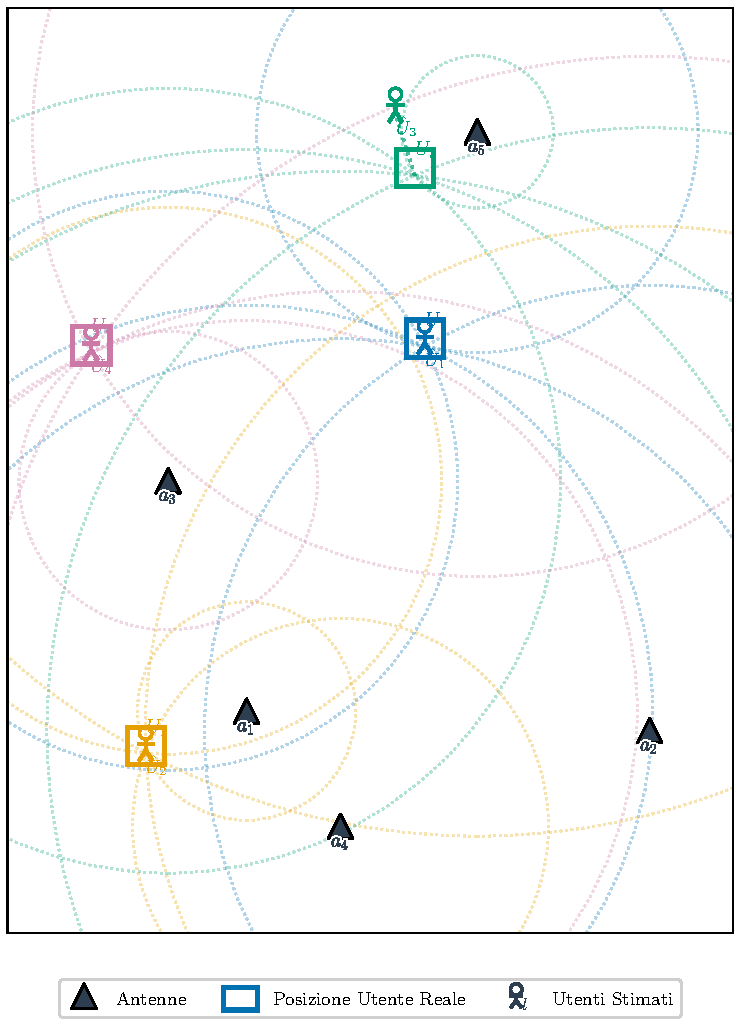
\includegraphics[width=1\textwidth]{Sources/Chapter4/figures/antenna_localization_plot.pdf}
	\caption{Stima della posizione degli utenti e delle antenne in assenza di rumore. I quadrati trasparenti indicano le posizioni reali degli utenti $U_r$, gli omini indicano le posizioni stimate $\hat{U}_r$, i triangoli scuri indicano le antenne $a_i$, e le circonferenze tratteggiate indicano le distanze stimate dalle antenne.}
	\label{fig:antenna_localization_plot}
\end{figure}

\begin{figure}[htbp]
	\centering
	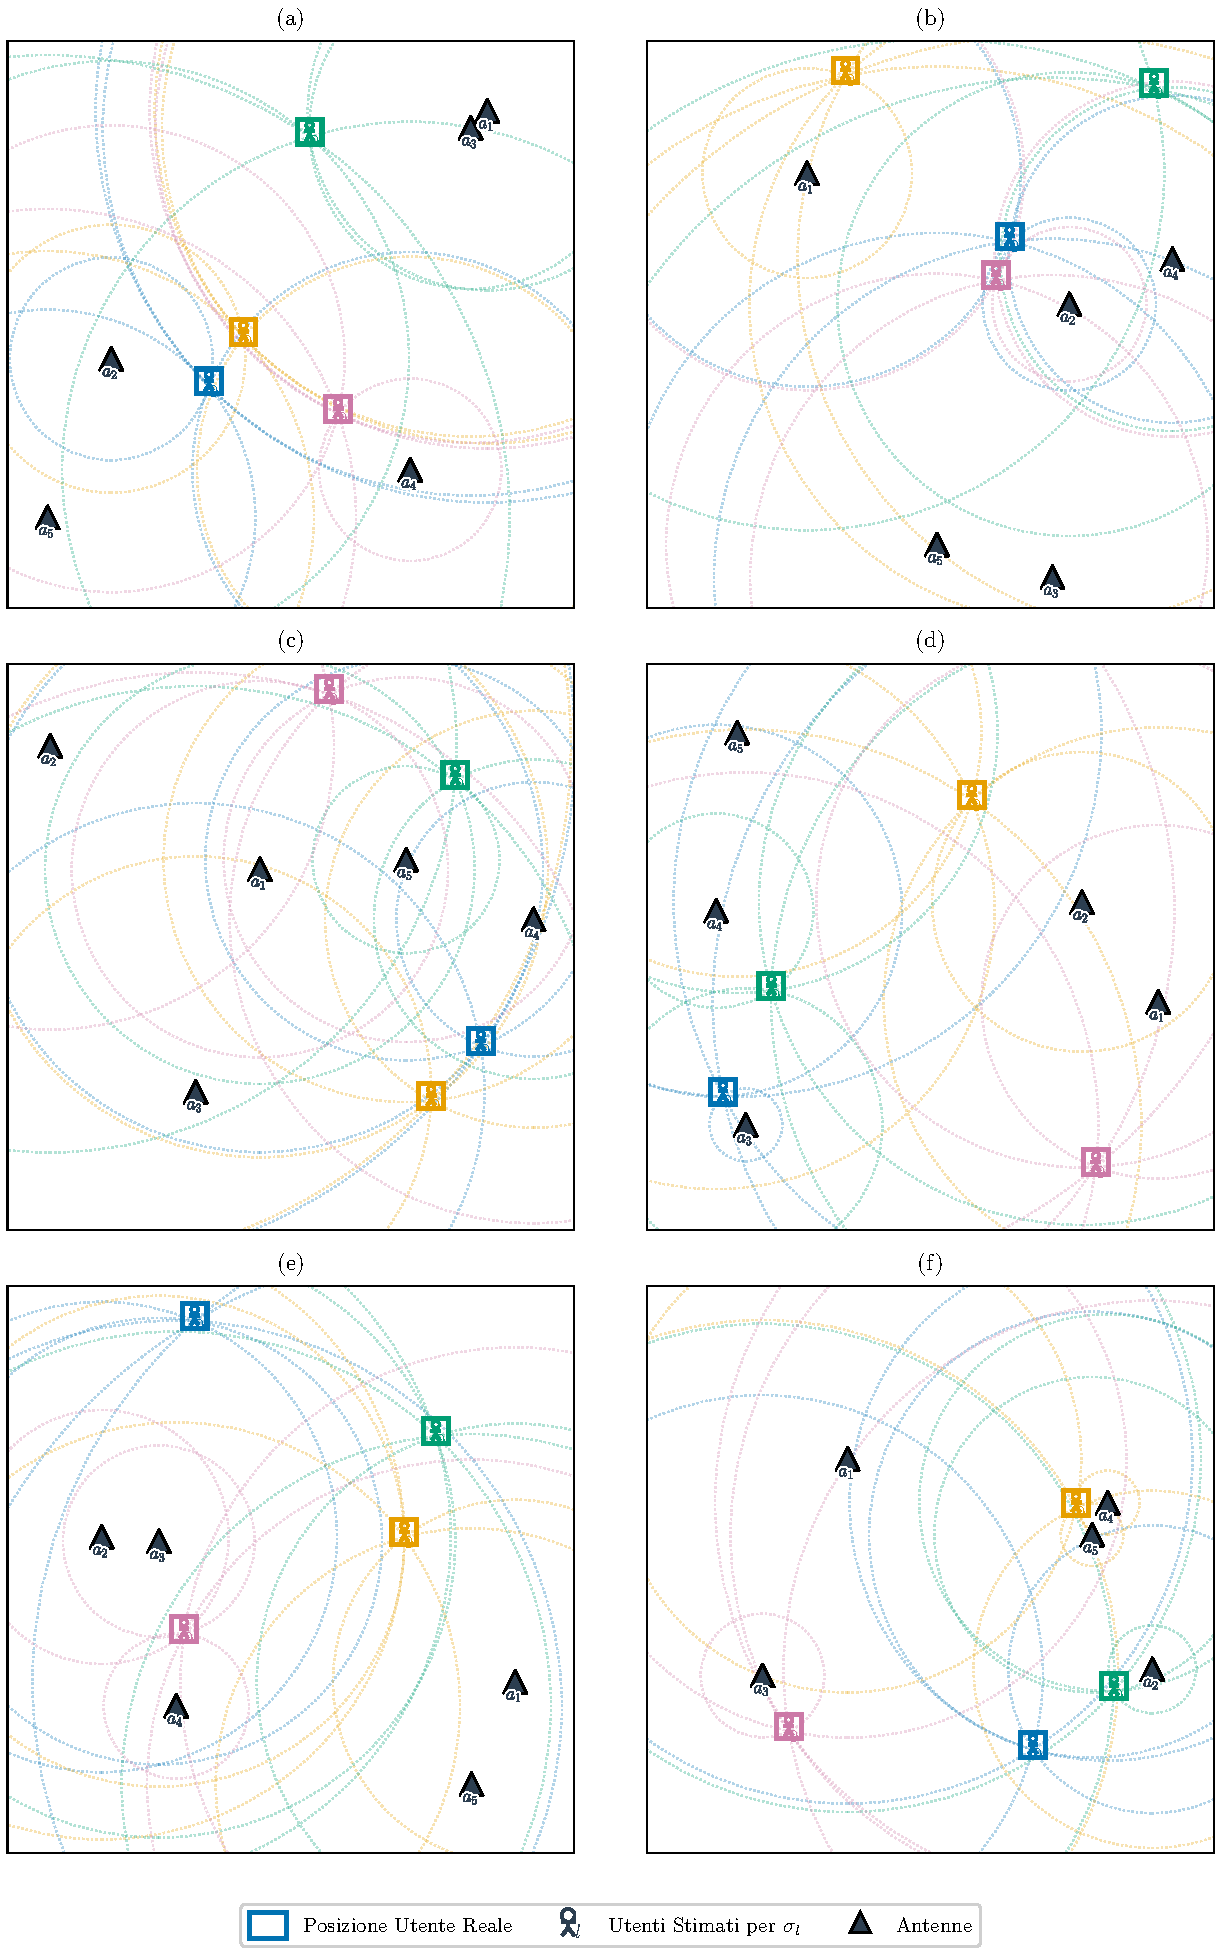
\includegraphics[width=\textwidth]{Sources/Chapter4/figures/dscdma_6_experiments.pdf}
	\caption{Stima della posizione degli utenti e delle antenne in sei esperimenti indipendenti con diverse disposizioni spaziali di antenne e sorgenti in assenza di rumore.}
	\label{fig:dscdma_6_experiments}
\end{figure}

\begin{figure}[htbp]
	\centering
	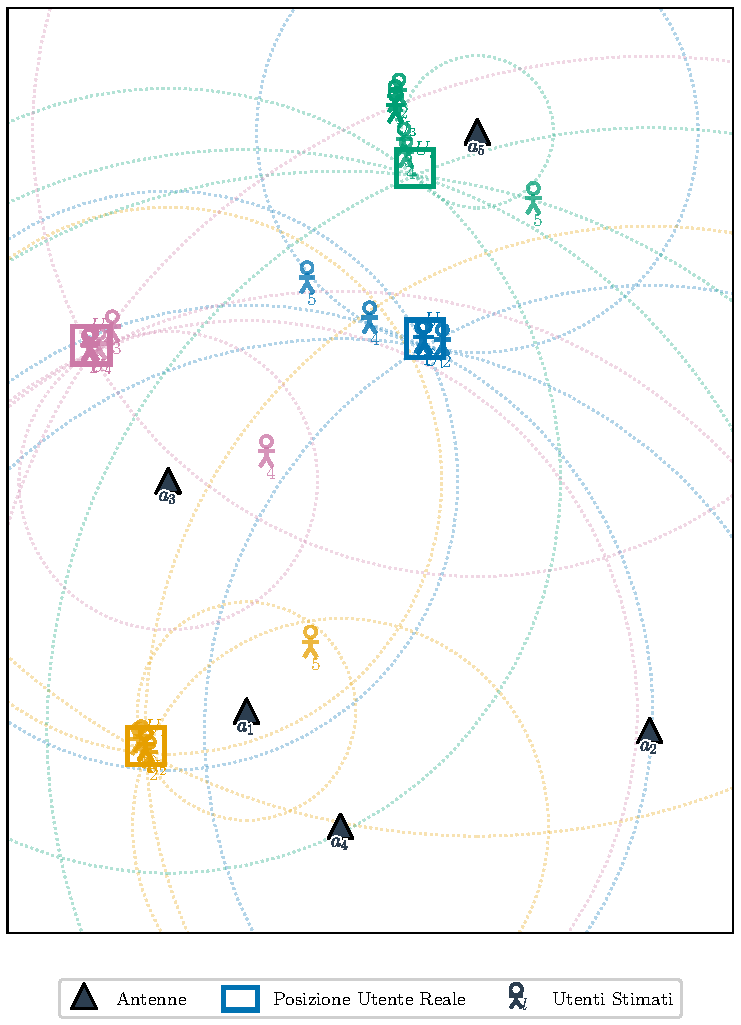
\includegraphics[width=\textwidth]{Sources/Chapter4/figures/dscdma_noise_experiment.pdf}
	\caption{Deriva della localizzazione degli utenti sotto sei livelli crescenti di rumore gaussiano ($\sigma_0, \ldots, \sigma_5$) per un singolo esperimento. Gli omini numerati da $1$ a $5$ indicano le posizioni stimate al crescere del livello di rumore.}
	\label{fig:dscdma_noise_experiment}
\end{figure}

\begin{figure}[htbp]
	\centering
	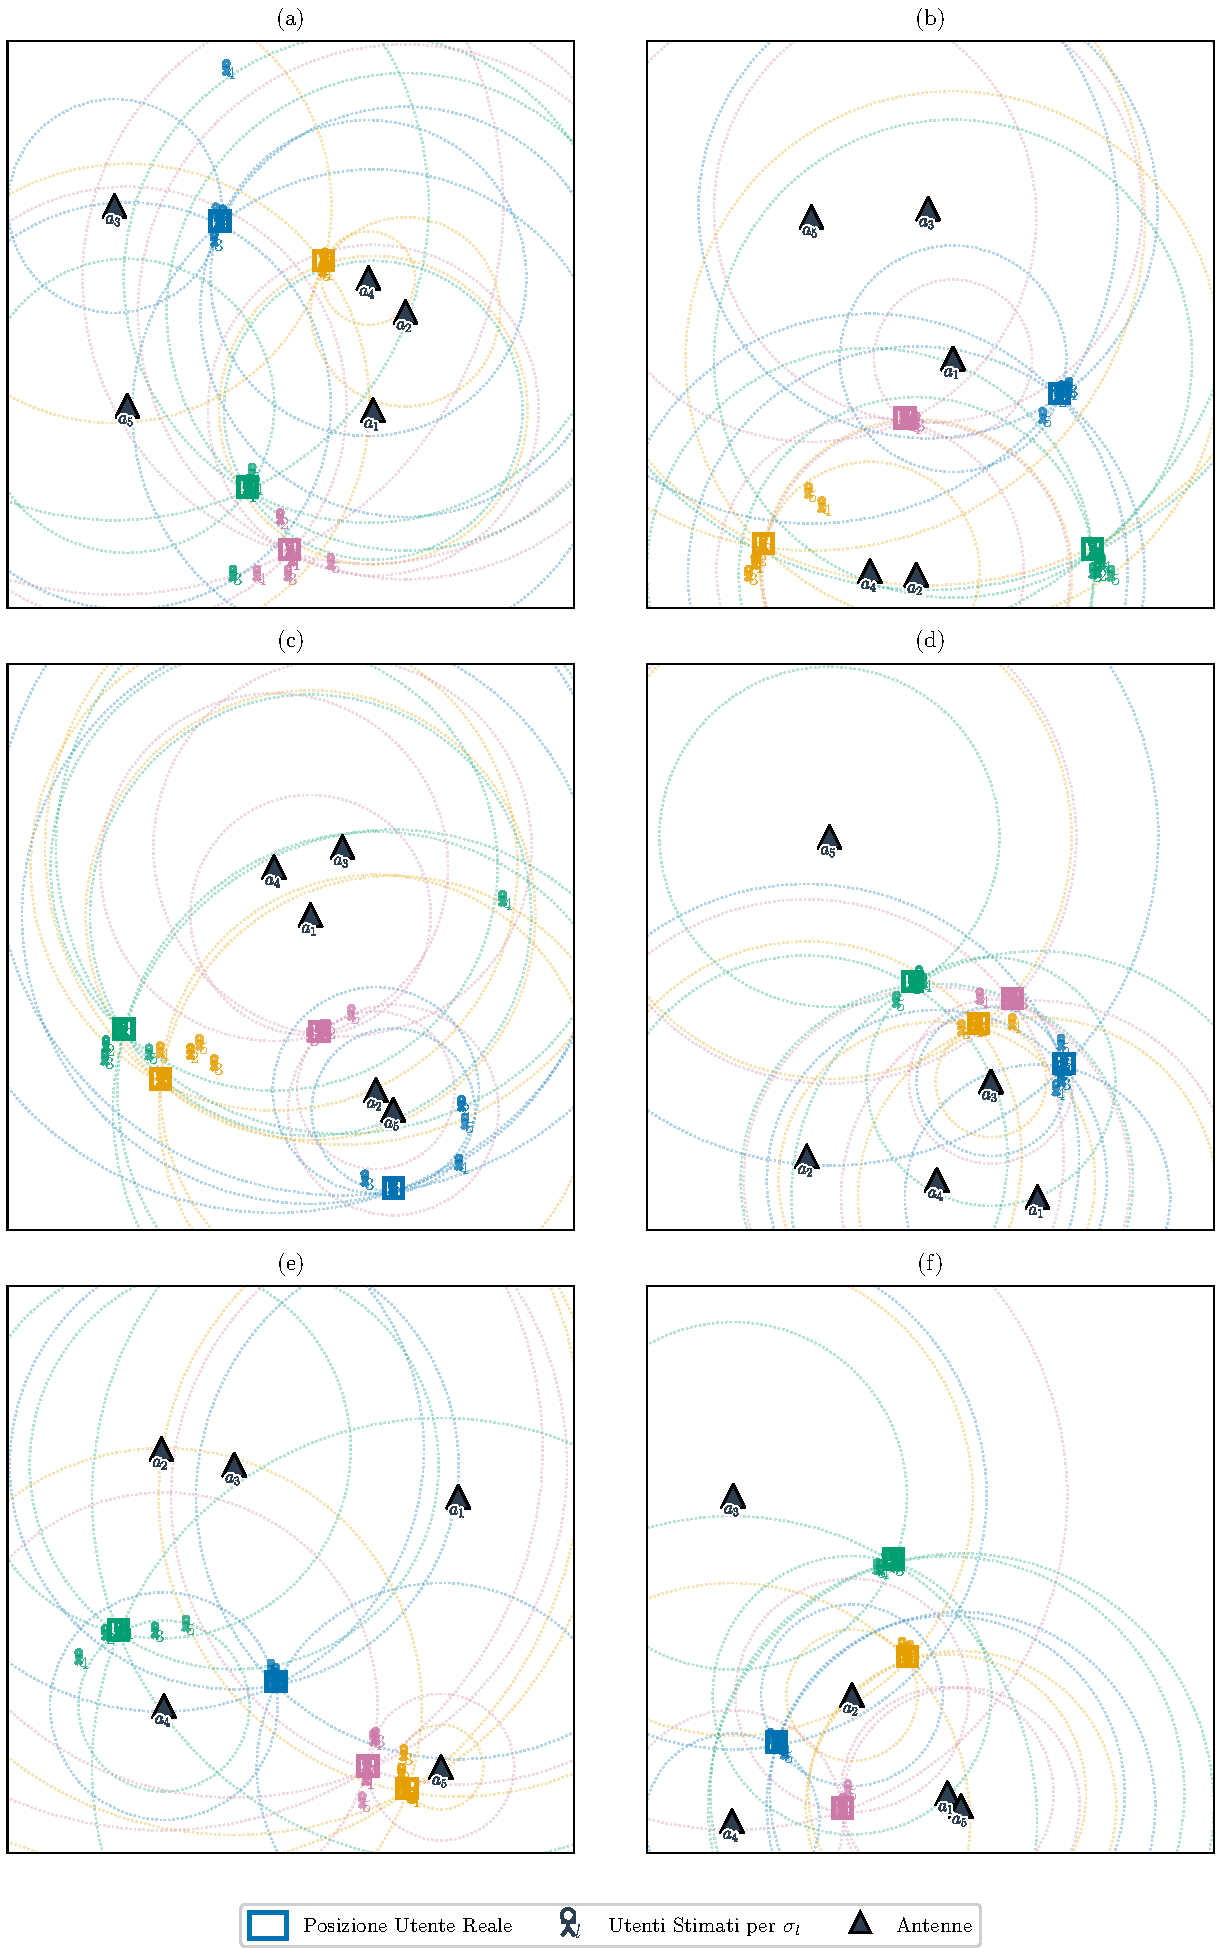
\includegraphics[width=\textwidth]{Sources/Chapter4/figures/dscdma_noise_experiment_multi.pdf}
	\caption{Deriva della localizzazione degli utenti sotto rumore gaussiano per sei esperimenti indipendenti (disposizioni spaziali differenti), mostrando i comportamenti tipici di deriva al crescere del livello di rumore $\sigma_l$.}
	\label{fig:dscdma_noise_experiment_multi}
\end{figure}
